% Options for packages loaded elsewhere
\PassOptionsToPackage{unicode}{hyperref}
\PassOptionsToPackage{hyphens}{url}
%
\documentclass[
  ignorenonframetext,
]{beamer}
\usepackage{pgfpages}
\setbeamertemplate{caption}[numbered]
\setbeamertemplate{caption label separator}{: }
\setbeamercolor{caption name}{fg=normal text.fg}
\beamertemplatenavigationsymbolsempty
% Prevent slide breaks in the middle of a paragraph
\widowpenalties 1 10000
\raggedbottom
\setbeamertemplate{part page}{
  \centering
  \begin{beamercolorbox}[sep=16pt,center]{part title}
    \usebeamerfont{part title}\insertpart\par
  \end{beamercolorbox}
}
\setbeamertemplate{section page}{
  \centering
  \begin{beamercolorbox}[sep=12pt,center]{part title}
    \usebeamerfont{section title}\insertsection\par
  \end{beamercolorbox}
}
\setbeamertemplate{subsection page}{
  \centering
  \begin{beamercolorbox}[sep=8pt,center]{part title}
    \usebeamerfont{subsection title}\insertsubsection\par
  \end{beamercolorbox}
}
\AtBeginPart{
  \frame{\partpage}
}
\AtBeginSection{
  \ifbibliography
  \else
    \frame{\sectionpage}
  \fi
}
\AtBeginSubsection{
  \frame{\subsectionpage}
}
\usepackage{amsmath,amssymb}
\usepackage{lmodern}
\usepackage{iftex}
\ifPDFTeX
  \usepackage[T1]{fontenc}
  \usepackage[utf8]{inputenc}
  \usepackage{textcomp} % provide euro and other symbols
\else % if luatex or xetex
  \usepackage{unicode-math}
  \defaultfontfeatures{Scale=MatchLowercase}
  \defaultfontfeatures[\rmfamily]{Ligatures=TeX,Scale=1}
\fi
% Use upquote if available, for straight quotes in verbatim environments
\IfFileExists{upquote.sty}{\usepackage{upquote}}{}
\IfFileExists{microtype.sty}{% use microtype if available
  \usepackage[]{microtype}
  \UseMicrotypeSet[protrusion]{basicmath} % disable protrusion for tt fonts
}{}
\makeatletter
\@ifundefined{KOMAClassName}{% if non-KOMA class
  \IfFileExists{parskip.sty}{%
    \usepackage{parskip}
  }{% else
    \setlength{\parindent}{0pt}
    \setlength{\parskip}{6pt plus 2pt minus 1pt}}
}{% if KOMA class
  \KOMAoptions{parskip=half}}
\makeatother
\usepackage{xcolor}
\IfFileExists{xurl.sty}{\usepackage{xurl}}{} % add URL line breaks if available
\IfFileExists{bookmark.sty}{\usepackage{bookmark}}{\usepackage{hyperref}}
\hypersetup{
  hidelinks,
  pdfcreator={LaTeX via pandoc}}
\urlstyle{same} % disable monospaced font for URLs
\newif\ifbibliography
\usepackage{graphicx}
\makeatletter
\def\maxwidth{\ifdim\Gin@nat@width>\linewidth\linewidth\else\Gin@nat@width\fi}
\def\maxheight{\ifdim\Gin@nat@height>\textheight\textheight\else\Gin@nat@height\fi}
\makeatother
% Scale images if necessary, so that they will not overflow the page
% margins by default, and it is still possible to overwrite the defaults
% using explicit options in \includegraphics[width, height, ...]{}
\setkeys{Gin}{width=\maxwidth,height=\maxheight,keepaspectratio}
% Set default figure placement to htbp
\makeatletter
\def\fps@figure{htbp}
\makeatother
\setlength{\emergencystretch}{3em} % prevent overfull lines
\providecommand{\tightlist}{%
  \setlength{\itemsep}{0pt}\setlength{\parskip}{0pt}}
\setcounter{secnumdepth}{-\maxdimen} % remove section numbering
\ifLuaTeX
  \usepackage{selnolig}  % disable illegal ligatures
\fi

\author{}
\date{\vspace{-2.5em}}

\begin{document}

\begin{frame}
\end{frame}

\begin{frame}{Mikroøkonomi med anvendelser (våren 2022)}
\protect\hypertarget{mikrouxf8konomi-med-anvendelser-vuxe5ren-2022}{}

\includegraphics{man/figures/abc.jpg}

\begin{block}{Nyheter}
\protect\hypertarget{nyheter}{}
Forelesningen skjer framover fysisk på Campus (Sone A Aud 2). Men jeg
har fått tillatelse av instituttleder til også legge ut en Zoom-lenke,
slik at vi har muligheten for en hybridløsning. Selve undervisningen vil
bli designet mest med tanke på de studentene som er fysisk tilstede, men
skal foresøke å ivarete begge hensyn.

\begin{itemize}
\tightlist
\item
  En del av materiale som ble benyttet under forelesninge \#2 er nå
  inkludert i forlesningsnotatene.
\end{itemize}
\end{block}

\begin{block}{Studietips}
\protect\hypertarget{studietips}{}
\href{https://github.com/joernih/SFB10816Mikrooekonomi/blob/main/inst/systemvsmaal.pdf}{Generelle
studietips\_ System framfor mål.pdf}
\end{block}

\begin{block}{Pensum}
\protect\hypertarget{pensum}{}

\includegraphics[width=0.2\textwidth,height=\textheight]{man/figures/pensum.jpg}
\href{https://www.cappelendammundervisning.no/_innforing-i-mikrookonomi-9788202640521}{Pensumbok
(Andreassen, Bredesen og Thøgersen)} 2. utgave (som må kjøpes brukt) kan
fortsatt benyttes, men 3. utgave er en vesentlig oppdatering (med blant
annet nye eksempler og bedre forklaringer)

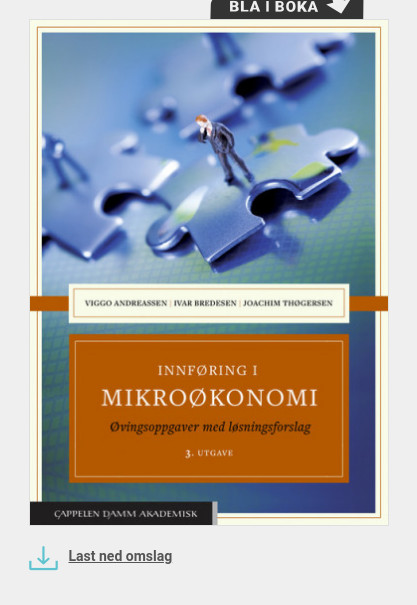
\includegraphics[width=0.1\textwidth,height=\textheight]{man/figures/oppgaver.jpg}

\href{https://www.cappelendammundervisning.no/_innforing-i-mikrookonomi-ovingsoppgaver-med-losningsforslag-9788202656485}{Oppgavebok
(Andreassen, Bredesen og Thøgersen)}

Undervisnings- og emneansvarlig (jornih at hiof.no)

Jørn I. Halvorsen

\textbf{Siste gang oppdatert: 2022-01-20 13:17:55}
\end{block}
\end{frame}

\end{document}
